\documentclass[16pt]{beamer}
\usepackage[utf8]{inputenc}
\usepackage[T1]{fontenc}
\usepackage{graphicx}
\usepackage[polish]{babel}
\usepackage{url}

% looks good at black background

\usepackage{fancyvrb}
\usepackage{color}

\makeatletter
\def\PY@reset{\let\PY@it=\relax \let\PY@bf=\relax%
    \let\PY@ul=\relax \let\PY@tc=\relax%
    \let\PY@bc=\relax \let\PY@ff=\relax}
\def\PY@tok#1{\csname PY@tok@#1\endcsname}
\def\PY@toks#1+{\ifx\relax#1\empty\else%
    \PY@tok{#1}\expandafter\PY@toks\fi}
\def\PY@do#1{\PY@bc{\PY@tc{\PY@ul{%
    \PY@it{\PY@bf{\PY@ff{#1}}}}}}}
\def\PY#1#2{\PY@reset\PY@toks#1+\relax+\PY@do{#2}}

\def\PY@tok@gd{\def\PY@tc##1{\textcolor[rgb]{0.63,0.00,0.00}{##1}}}
\def\PY@tok@gu{\let\PY@bf=\textbf\def\PY@tc##1{\textcolor[rgb]{0.50,0.00,0.50}{##1}}}
\def\PY@tok@gt{\def\PY@tc##1{\textcolor[rgb]{0.00,0.25,0.82}{##1}}}
\def\PY@tok@gs{\let\PY@bf=\textbf}
\def\PY@tok@gr{\def\PY@tc##1{\textcolor[rgb]{1.00,0.00,0.00}{##1}}}
\def\PY@tok@cm{\let\PY@it=\textit\def\PY@tc##1{\textcolor[rgb]{0.00,0.53,0.00}{##1}}}
\def\PY@tok@vg{\def\PY@tc##1{\textcolor[rgb]{0.72,0.53,0.04}{##1}}}
\def\PY@tok@m{\def\PY@tc##1{\textcolor[rgb]{0.40,0.40,0.40}{##1}}}
\def\PY@tok@mh{\def\PY@tc##1{\textcolor[rgb]{0.40,0.40,0.40}{##1}}}
\def\PY@tok@cs{\let\PY@bf=\textbf\def\PY@tc##1{\textcolor[rgb]{0.00,0.53,0.00}{##1}}}
\def\PY@tok@ge{\let\PY@it=\textit}
\def\PY@tok@vc{\def\PY@tc##1{\textcolor[rgb]{0.72,0.53,0.04}{##1}}}
\def\PY@tok@il{\def\PY@tc##1{\textcolor[rgb]{0.40,0.40,0.40}{##1}}}
\def\PY@tok@go{\def\PY@tc##1{\textcolor[rgb]{0.50,0.50,0.50}{##1}}}
\def\PY@tok@cp{\def\PY@tc##1{\textcolor[rgb]{0.00,0.53,0.00}{##1}}}
\def\PY@tok@gi{\def\PY@tc##1{\textcolor[rgb]{0.00,0.63,0.00}{##1}}}
\def\PY@tok@gh{\let\PY@bf=\textbf\def\PY@tc##1{\textcolor[rgb]{0.00,0.00,0.50}{##1}}}
\def\PY@tok@ni{\let\PY@bf=\textbf\def\PY@tc##1{\textcolor[rgb]{0.60,0.60,0.60}{##1}}}
\def\PY@tok@nl{\def\PY@tc##1{\textcolor[rgb]{0.63,0.63,0.00}{##1}}}
\def\PY@tok@nn{\let\PY@bf=\textbf\def\PY@tc##1{\textcolor[rgb]{0.00,0.00,1.00}{##1}}}
\def\PY@tok@no{\def\PY@tc##1{\textcolor[rgb]{0.53,0.00,0.00}{##1}}}
\def\PY@tok@na{\def\PY@tc##1{\textcolor[rgb]{0.73,0.27,0.27}{##1}}}
\def\PY@tok@nb{\def\PY@tc##1{\textcolor[rgb]{0.67,0.13,1.00}{##1}}}
\def\PY@tok@nc{\def\PY@tc##1{\textcolor[rgb]{0.00,0.00,1.00}{##1}}}
\def\PY@tok@nd{\def\PY@tc##1{\textcolor[rgb]{0.67,0.13,1.00}{##1}}}
\def\PY@tok@ne{\let\PY@bf=\textbf\def\PY@tc##1{\textcolor[rgb]{0.82,0.25,0.23}{##1}}}
\def\PY@tok@nf{\def\PY@tc##1{\textcolor[rgb]{0.00,0.63,0.00}{##1}}}
\def\PY@tok@si{\let\PY@bf=\textbf\def\PY@tc##1{\textcolor[rgb]{0.73,0.40,0.53}{##1}}}
\def\PY@tok@s2{\def\PY@tc##1{\textcolor[rgb]{0.73,0.27,0.27}{##1}}}
\def\PY@tok@vi{\def\PY@tc##1{\textcolor[rgb]{0.72,0.53,0.04}{##1}}}
\def\PY@tok@nt{\let\PY@bf=\textbf\def\PY@tc##1{\textcolor[rgb]{0.00,0.50,0.00}{##1}}}
\def\PY@tok@nv{\def\PY@tc##1{\textcolor[rgb]{0.72,0.53,0.04}{##1}}}
\def\PY@tok@s1{\def\PY@tc##1{\textcolor[rgb]{0.73,0.27,0.27}{##1}}}
\def\PY@tok@gp{\let\PY@bf=\textbf\def\PY@tc##1{\textcolor[rgb]{0.00,0.00,0.50}{##1}}}
\def\PY@tok@sh{\def\PY@tc##1{\textcolor[rgb]{0.73,0.27,0.27}{##1}}}
\def\PY@tok@ow{\let\PY@bf=\textbf\def\PY@tc##1{\textcolor[rgb]{0.67,0.13,1.00}{##1}}}
\def\PY@tok@sx{\def\PY@tc##1{\textcolor[rgb]{0.00,0.50,0.00}{##1}}}
\def\PY@tok@bp{\def\PY@tc##1{\textcolor[rgb]{0.67,0.13,1.00}{##1}}}
\def\PY@tok@c1{\let\PY@it=\textit\def\PY@tc##1{\textcolor[rgb]{0.00,0.53,0.00}{##1}}}
\def\PY@tok@kc{\let\PY@bf=\textbf\def\PY@tc##1{\textcolor[rgb]{0.67,0.13,1.00}{##1}}}
\def\PY@tok@c{\let\PY@it=\textit\def\PY@tc##1{\textcolor[rgb]{0.00,0.53,0.00}{##1}}}
\def\PY@tok@mf{\def\PY@tc##1{\textcolor[rgb]{0.40,0.40,0.40}{##1}}}
\def\PY@tok@err{\def\PY@bc##1{\fcolorbox[rgb]{1.00,0.00,0.00}{1,1,1}{##1}}}
\def\PY@tok@kd{\let\PY@bf=\textbf\def\PY@tc##1{\textcolor[rgb]{0.67,0.13,1.00}{##1}}}
\def\PY@tok@ss{\def\PY@tc##1{\textcolor[rgb]{0.72,0.53,0.04}{##1}}}
\def\PY@tok@sr{\def\PY@tc##1{\textcolor[rgb]{0.73,0.40,0.53}{##1}}}
\def\PY@tok@mo{\def\PY@tc##1{\textcolor[rgb]{0.40,0.40,0.40}{##1}}}
\def\PY@tok@mi{\def\PY@tc##1{\textcolor[rgb]{0.40,0.40,0.40}{##1}}}
\def\PY@tok@kn{\let\PY@bf=\textbf\def\PY@tc##1{\textcolor[rgb]{0.67,0.13,1.00}{##1}}}
\def\PY@tok@o{\def\PY@tc##1{\textcolor[rgb]{0.40,0.40,0.40}{##1}}}
\def\PY@tok@kr{\let\PY@bf=\textbf\def\PY@tc##1{\textcolor[rgb]{0.67,0.13,1.00}{##1}}}
\def\PY@tok@s{\def\PY@tc##1{\textcolor[rgb]{0.73,0.27,0.27}{##1}}}
\def\PY@tok@kp{\def\PY@tc##1{\textcolor[rgb]{0.67,0.13,1.00}{##1}}}
\def\PY@tok@w{\def\PY@tc##1{\textcolor[rgb]{0.73,0.73,0.73}{##1}}}
\def\PY@tok@kt{\let\PY@bf=\textbf\def\PY@tc##1{\textcolor[rgb]{0.00,0.73,0.00}{##1}}}
\def\PY@tok@sc{\def\PY@tc##1{\textcolor[rgb]{0.73,0.27,0.27}{##1}}}
\def\PY@tok@sb{\def\PY@tc##1{\textcolor[rgb]{0.73,0.27,0.27}{##1}}}
\def\PY@tok@k{\let\PY@bf=\textbf\def\PY@tc##1{\textcolor[rgb]{0.67,0.13,1.00}{##1}}}
\def\PY@tok@se{\let\PY@bf=\textbf\def\PY@tc##1{\textcolor[rgb]{0.73,0.40,0.13}{##1}}}
\def\PY@tok@sd{\let\PY@it=\textit\def\PY@tc##1{\textcolor[rgb]{0.73,0.27,0.27}{##1}}}

\def\PYZbs{\char`\\}
\def\PYZus{\char`\_}
\def\PYZob{\char`\{}
\def\PYZcb{\char`\}}
\def\PYZca{\char`\^}
% for compatibility with earlier versions
\def\PYZat{@}
\def\PYZlb{[}
\def\PYZrb{]}
\makeatother


\usetheme{Pittsburgh}
\usecolortheme{seahorse}
\setbeamertemplate{items}[ball]

\beamertemplatesolidbackgroundcolor{black}
\setbeamercolor{normal text}{fg=white}

\usenavigationsymbolstemplate{} % turn off navigation icons

\author{Silesian Ruby Users Group\\
  \footnotesize{Wojciech Wnętrzak}}
\date{December 3, 2010}
\title{Introduction to "Chef" framework}

\begin{document}

\frame{\titlepage}

\begin{frame}
  \frametitle{What Is Chef?}
  \begin{itemize}
    \item Open Source (Apache License v. 2.0)
    \item Framework
    \item Ruby
  \end{itemize}
\end{frame}

\begin{frame}
  \frametitle{Chef Is Young}
  \begin{itemize}
    \item Released on January 15th, 2009
  \end{itemize}
  \begin{figure}
    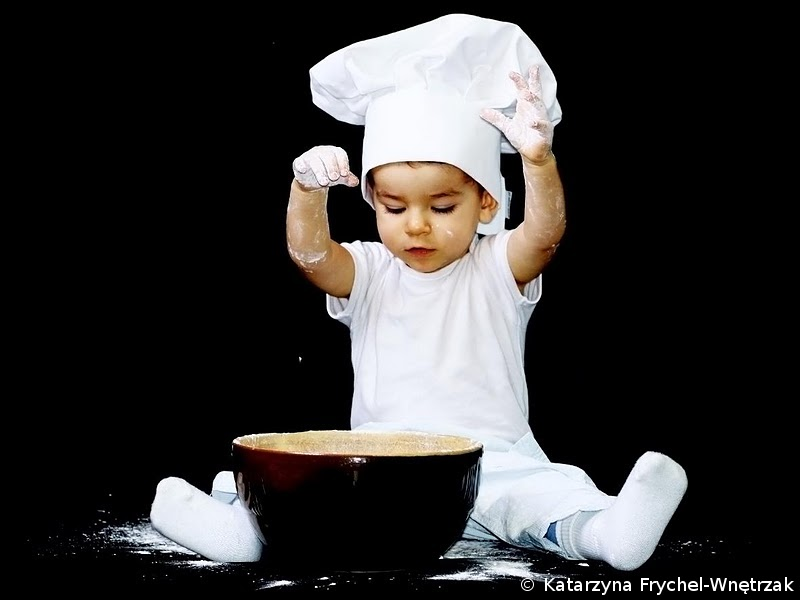
\includegraphics[width=0.8\linewidth]{images/young-chef}
  \end{figure}
\end{frame}

\begin{frame}
  \frametitle{Why To Use Chef?}
  \begin{itemize}
    \item Only one administration guy in company?
    \item Forces order in system
    \item Existing solutions for your problems
    \item Best practices
  \end{itemize}
\end{frame}

\begin{frame}
  \frametitle{How To Use Chef?}
  \begin{itemize}
    \item \emph{chef-client} + \emph{chef-server}
    \item \emph{chef-client} + Opscode Platform
    \item \emph{chef-solo}
  \end{itemize}
\end{frame}

\begin{frame}
  \frametitle{Chef Server}
  \begin{itemize}
    \item Ruby gem (\emph{chef-server})
    \item Stores cookbooks
    \item Stores information about nodes
    \item Accessbile by REST API
  \end{itemize}
\end{frame}

\begin{frame}
  \frametitle{Chef Server Elements}
  \begin{itemize}
    \item CouchDB -- stores node informations
    \item SOLR -- data indexing
    \item RabbitMQ -- helps in indexing
    \item Merb -- API and web user interface
  \end{itemize}
  \pause
  \begin{center}
    \LARGE \color{red} That is lot of stuff!
  \end{center}
\end{frame}

\begin{frame}
  \frametitle{Opscode Platform}
  \begin{itemize}
    \item Free plan (upto 5 nodes)
    \item Configuration step by step
    \item Organizations and users managment
  \end{itemize}
\end{frame}

\begin{frame}
  \frametitle{Chef Client}
  \begin{itemize}
    \item Ruby gem (\emph{chef})
    \item Runs on machine that we want to configure
    \item Communicates with chef server
  \end{itemize}
\end{frame}

\begin{frame}
  \frametitle{Chef Solo}
  \begin{itemize}
    \item Part of \emph{chef} gem
    \item Standalone run (without connecting to server)
    \item Uses cookbooks from local tarballs
  \end{itemize}
\end{frame}

\begin{frame}
  \frametitle{Simple Workflow}
  \begin{itemize}
    \item Write cookbook with recipe
    \item Upload it to chef server
    \item Define run list by:
    \begin{description}
      \item{---} editing node on chef server
      \item{---} passing JSON file to chef-client
    \end{description}
    \item Run chef-client on desired machine
  \end{itemize}
\end{frame}

\begin{frame}
  \frametitle{Cookbooks}
  \begin{center}
    \LARGE ''Cookbooks for Chef are like RubyGems for Ruby''\footnote{I couldn't find author}
  \end{center}
\end{frame}

\begin{frame}
  \frametitle{Cookbook Skeleton}
  \begin{figure}
    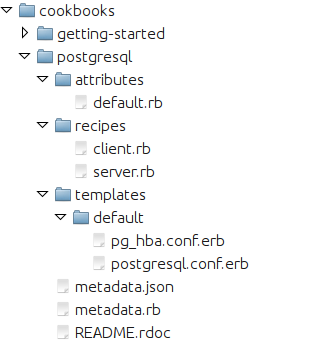
\includegraphics[width=0.6\linewidth]{images/cookbook-skeleton}
  \end{figure}
\end{frame}

\begin{frame}
  \frametitle{Example Attributes File}
  \begin{footnotesize}
    \input{listing/postgres_attributes}
    \label{postgres_attributes}
  \end{footnotesize}
\end{frame}

\begin{frame}
  \frametitle{Example Recipe File}
  \begin{footnotesize}
    \input{listing/postgres_server_recipe}
    \label{postgres_server_recipe}
    \end{footnotesize}
\end{frame}

\begin{frame}
  \frametitle{Package Providers}
  \begin{itemize}
    \item Apt
    \item Yum
    \item MacPorts
  \end{itemize}
  \pause
  \begin{center}
    \large Many more
  \end{center}
\end{frame}

\begin{frame}
  \frametitle{Supported Systems}
  \begin{itemize}
    \item Debian
    \item Gentoo
    \item FreeBSD
    \item MacOSX
    \item Solaris
    \pause
    \item Windows
  \end{itemize}
  \pause
  \begin{center}
    \large And more
  \end{center}
\end{frame}

\begin{frame}
  \frametitle{Resources\footnote{\url{http://wiki.opscode.com/display/chef/Resources}}}
  \begin{itemize}
    \item package
    \item template
    \item file
    \item user
    \item execute
    \item script (bash, ruby, perl, python, csh)
    \item http\_request
    \item deploy
  \end{itemize}
  \pause
  \begin{center}
    \large Many more
  \end{center}
\end{frame}

\begin{frame}
  \frametitle{Additional Tools - Ohai}
  \begin{itemize}
    \item Released as a gem -- \emph{ohai}
    \item Collects system configuration/information
    \item Returns \emph{JSON}
  \end{itemize}
\end{frame}

\begin{frame}
  \frametitle{Additional Tools - Knife}
  \begin{itemize}
    \item Part of \emph{chef} gem
    \item Console tool for chef server managment
  \end{itemize}
\end{frame}

\begin{frame}
  \frametitle{Tips}
  \begin{itemize}
    \item If using \emph{RVM}, use \emph{rvmsudo} for \emph{chef-client}
    \item Take a look at chef bootstrap\footnote{\url{http://wiki.opscode.com/display/chef/Bootstrap+Chef+RubyGems+Installation}}
    \item Remember that Ruby (Chef) uses \emph{sh}, not \emph{bash}
  \end{itemize}
\end{frame}

\begin{frame}
  \frametitle{Useful Links}
  \begin{footnotesize}
    \begin{itemize}
      \item \url{http://www.opscode.com/chef/}
      \item \url{http://help.opscode.com/faqs/start/how-to-get-started}
      \item \url{https://github.com/opscode/cookbooks}
    \end{itemize}
  \end{footnotesize}
\end{frame}

\begin{frame}
  \frametitle{Thank You}
  \begin{center}
    \Huge Questions?
  \end{center}
\end{frame}

\end{document}
